\documentclass{beamer}

\mode<presentation>
\usepackage{amsmath,amssymb,mathtools}
\usepackage{textcomp}
\usepackage{gensymb}
\usepackage{adjustbox}
\usepackage{subcaption}
\usepackage{enumitem}
\usepackage[utf8]{inputenc}
\usepackage{amssymb}
\usepackage{newunicodechar}
\usepackage{enumitem}
\setlist{nosep} % optional: removes vertical gaps
\setlist[enumerate]{label=\arabic*)} % custom numbering if you want

\newunicodechar{√}{$\sqrt{\;}$}
\newunicodechar{✅}{\checkmark}
\newunicodechar{❌}{\texttimes}
\usepackage{multicol}
\usepackage{listings}
\usepackage{url}
\usepackage{graphicx} % <-- needed for images
\def\UrlBreaks{\do\/\do-}

\usetheme{Boadilla}
\usecolortheme{lily}
\setbeamertemplate{footline}{
  \leavevmode%
  \hbox{%
  \begin{beamercolorbox}[wd=\paperwidth,ht=2ex,dp=1ex,right]{author in head/foot}%
    \insertframenumber{} / \inserttotalframenumber\hspace*{2ex}
  \end{beamercolorbox}}%
  \vskip0pt%
}
\setbeamertemplate{navigation symbols}{}

\lstset{
  frame=single,
  breaklines=true,
  columns=fullflexible,
  basicstyle=\ttfamily\tiny   % tiny font so code fits
}

\numberwithin{equation}{section}

% ---- your macros ----
\providecommand{\nCr}[2]{\,^{#1}{#2}}
\providecommand{\nPr}[2]{\,^{#1}P_{#2}}
\providecommand{\mbf}{\mathbf}
\providecommand{\pr}[1]{\ensuremath{\Pr\left(#1\right)}}
\providecommand{\qfunc}[1]{\ensuremath{Q\left(#1\right)}}
\providecommand{\sbrak}[1]{\ensuremath{{}\left[#1\right]}}
\providecommand{\lsbrak}[1]{\ensuremath{{}\left[#1\right.}}
\providecommand{\rsbrak}[1]{\ensuremath{\left.#1\right]}}
\providecommand{\brak}[1]{\ensuremath{\left(#1\right)}}
\providecommand{\lbrak}[1]{\ensuremath{\left(#1\right.}}
\providecommand{\rbrak}[1]{\ensuremath{\left.#1\right)}}
\providecommand{\cbrak}[1]{\ensuremath{\left\{#1\right\}}}
\providecommand{\lcbrak}[1]{\ensuremath{\left\{#1\right.}}
\providecommand{\rcbrak}[1]{\ensuremath{\left.#1\right\}}}
\theoremstyle{remark}
\newtheorem{rem}{Remark}
\newcommand{\sgn}{\mathop{\mathrm{sgn}}}
\providecommand{\abs}[1]{\left\vert#1\right\vert}
\providecommand{\res}[1]{\Res\displaylimits_{#1}}
\providecommand{\norm}[1]{\lVert#1\rVert}
\providecommand{\mtx}[1]{\mathbf{#1}}
\providecommand{\mean}[1]{E\left[ #1 \right]}
\providecommand{\fourier}{\overset{\mathcal{F}}{ \rightleftharpoons}}
\providecommand{\system}{\overset{\mathcal{H}}{ \longleftrightarrow}}
\providecommand{\dec}[2]{\ensuremath{\overset{#1}{\underset{#2}{\gtrless}}}}
\newcommand{\myvec}[1]{\ensuremath{\begin{pmatrix}#1\end{pmatrix}}}
\let\vec\mathbf
% ---------------------

\title{Matgeo Presentation - Problem 5.8.19}
\author{ee25btech11021 - Dhanush sagar}

\begin{document}
	

		




%---------------- Title Page ----------------
\begin{frame}
  \titlepage
\end{frame}

%---------------- Problem Statement ----------------
\begin{frame}{Problem Statement}
If we add 1 to the numerator and subtract 1 from the denominator, a fraction reduces
to 1. It becomes 1/2 if we only add 1 to the denominator. What is the fraction?
\end{frame}

%---------------- Mathematical Formula ----------------
\begin{frame}{solution}

Let the unknown fraction be represented as
\begin{align}
\vec{u} &= \myvec{x \\ y}, \qquad 
\frac{x}{y}.
\end{align}

Affine transformations are written as a vector plus a translation.\\

case 1:add 1 to numerator, subtract 1 from denominator
\begin{align}
T_1(\vec{u}) &= \vec{u} + \myvec{1 \\ -1}, \quad 
\end{align}

case 2:add 1 to denominator
\begin{align}
T_2(\vec{u}) &= \vec{u} + \myvec{0 \\ 1}, \quad
\end{align}

Condition for a fraction:  
For any vector $\myvec{a \\ b}$, the requirement $\tfrac{a}{b}=k$ is equivalent to the linear equation
\begin{align}
\vec{r}_k \myvec{a \\ b} = 0, 
\qquad \vec{r}_k = \myvec{1 & -k},
\end{align}
\end{frame}
\begin{frame}{solution}
since $\vec{r}_k \myvec{a \\ b} = a - kb = 0 \iff \tfrac{a}{b}=k$.



Case 1: $T_1(\vec{u})$ must yield fraction $1$.use $\vec{r}_1 = \myvec{1 & -1}$
\begin{align}
\vec{r}_1 \big(T_1(\vec{u})\big) &= 0 \\
\implies \vec{r}_1\vec{u} + \vec{r}_1\myvec{1 \\ -1} &= 0 \\
\myvec{1 & -1}\vec{u} + 2 &= 0 
\end{align}
This gives the first equation.



Case 2: $T_2(\vec{u})$ must yield fraction $\tfrac{1}{2}$.  
To avoid fractions, multiply the functional by $2$, i.e., use $\vec{r}_2 = \myvec{2 & -1}$.
\begin{align}
\vec{r}_2 \big(T_2(\vec{u})\big) &= 0 \\
\implies \vec{r}_2\vec{u} + \vec{r}_2\myvec{0 \\ 1} &= 0 \\
\myvec{2 & -1}\vec{u} - 1 &= 0 
\end{align}
This gives the second equation.

\end{frame}
\begin{frame}{solution}
System of equations:  
Both conditions together form the system
\begin{align}
\myvec{1 & -1 \\ 2 & -1}\vec{u} &= \myvec{-2 \\ 1}.
\end{align}



Gaussian elimination:  
Form the augmented matrix
\begin{align}
\left[\myvec{1 & -1 \\ 2 & -1} \;\middle|\; \myvec{-2 \\ 1}\right].
\end{align}
Eliminate the entry below the pivot:
\begin{align}
R_2 \leftarrow R_2 - 2R_1 \;\;\Rightarrow\;\;
\left[\myvec{1 & -1 \\ 0 & 1} \;\middle|\; \myvec{-2 \\ 5}\right].
\end{align}
Now eliminate above the pivot:
\begin{align}
R_1 \leftarrow R_1 + R_2 \;\;\Rightarrow\;\;
\left[\myvec{1 & 0 \\ 0 & 1} \;\middle|\; \myvec{3 \\ 5}\right].
\end{align}



Final solution:
\begin{align}
\vec{u} &= \myvec{3 \\ 5}, 
\frac{x}{y} = \frac{3}{5}.
\end{align}
\end{frame}
%---------------- C Source Code ----------------
\begin{frame}[fragile]{C Source Code:fraction matrix.c}
\begin{verbatim}
#include <stdio.h>

// Generate augmented matrix for fraction problem
void generate_matrix(double matrix[2][3]) {
    // Equation 1: x - y = -2
    matrix[0][0] = 1;
    matrix[0][1] = -1;
    matrix[0][2] = -2;

    // Equation 2: 2x - y = 1
    matrix[1][0] = 2;
    matrix[1][1] = -1;
    matrix[1][2] = 1;
}




\end{verbatim}
\end{frame}

%---------------- Python solve.py ----------------
\begin{frame}[fragile]{Python Script:fraction matrix.py}
\begin{verbatim}
import ctypes
import numpy as np

# Load the shared library
lib = ctypes.CDLL("./libfraction_matrix.so")

# Prepare 2x3 matrix
MatrixType = ctypes.c_double * 3 * 2
matrix = MatrixType()

# Call C function to generate matrix
lib.generate_matrix(matrix)



\end{verbatim}
\end{frame}

\begin{frame}[fragile]{Python Script:fraction matrix.py}
\begin{verbatim}
# Convert to numpy array
aug_matrix = np.array([[matrix[i][j] for j in range(3)] for i in range(2)])

# Solve system
A = aug_matrix[:, :2]
B = aug_matrix[:, 2]
solution = np.linalg.solve(A, B)
x, y = solution

print(f"The fraction is {x}/{y}")

# Optionally save fraction to file for plotting
with open("fraction.txt", "w") as f:
    f.write(f"{x} {y}")

\end{verbatim}
\end{frame}

\begin{frame}[fragile]{Python Script: plot matrix.py}
\begin{verbatim}
import numpy as np
import matplotlib.pyplot as plt

# Load fraction solution
with open("fraction.txt", "r") as f:
    x_sol, y_sol = map(float, f.read().split())

# Define the two lines from the equations:
# Equation 1: x - y = -2 → y = x + 2
# Equation 2: 2x - y = 1 → y = 2x - 1

x_vals = np.linspace(0, 5, 100)
y1 = x_vals + 2
y2 = 2*x_vals - 1



\end{verbatim}
\end{frame}
\begin{frame}[fragile]{Python Script: plot matrix.py}
\begin{verbatim}
# Plot the lines
plt.plot(x_vals, y1, label="x - y = -2")
plt.plot(x_vals, y2, label="2x - y = 1")

# Plot the intersection point
plt.scatter(x_sol, y_sol, color='red', s=100, label=f'Intersection ({x_sol},{y_sol})')

plt.xlabel("x (Numerator)")
plt.ylabel("y (Denominator)")
plt.title("Intersection of Two Lines (Fraction Solution)")
plt.grid(True)
plt.legend()
plt.show()
\end{verbatim}
\end{frame}

%---------------- Result Plot ----------------
\begin{frame}{Result Plot}
 \begin{figure}[H]
     \centering
     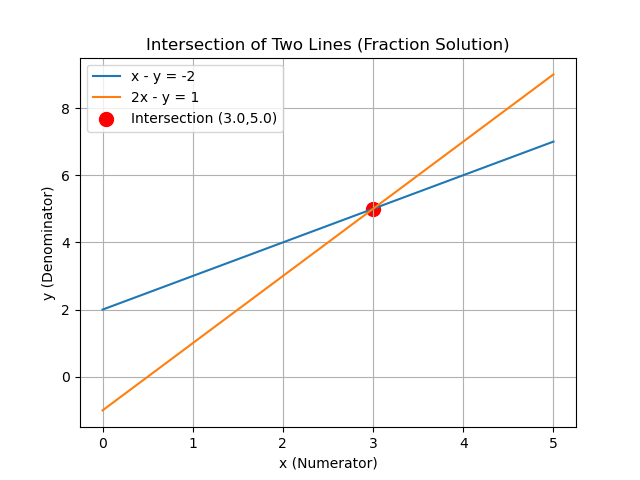
\includegraphics[width=0.7\columnwidth]{figs/fig1.png}
     \caption*{}
     \label{fig:fig1}
 \end{figure}
 
\end{frame}

\end{document}
